\documentclass[11pt]{beamer}
\usepackage[utf8]{inputenc}
\usepackage[T1]{fontenc}
%\usepackage{natbib}
\usetheme{Pittsburgh}
\usepackage{verbatim} 
\usepackage[english]{babel}
\usepackage{epstopdf}
\usepackage{hyperref}
\hypersetup{
colorlinks=true}
%\titlegraphic{%\vspace*{1cm}
%	\includegraphics[width=2.5cm]{logo_udelar}
	%\hspace*{1cm}~%
%		\includegraphics[width=3.5cm]{logo_FCEA.png}
%}
\setbeamertemplate{navigation symbols}{}
\setbeamertemplate{footline}[frame number]
\AtBeginSection{ 
	\begin{frame}
		\frametitle{Index}
			\tableofcontents[currentsection]
	\end{frame}
}
\begin{document}
	\title{Modelos dinámicos y computacionales en Economía}
	\subtitle{Coordinación en Sistemas Complejos}
%\logo{}
\institute{Licenciatura en Economía, FCEA, UDELAR}
\date{7 de noviembre de 2023}

	%\subject{}
	%\setbeamercovered{transparent}
	%\setbeamertemplate{navigation symbols}{}
	\frame[plain]{
	\begin{figure}
	\centering
	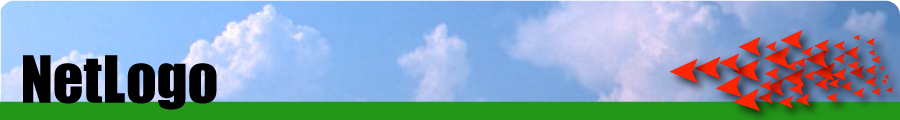
\includegraphics[width=0.7\linewidth]{figuras/netlogo-title-wide-60}
	%		\caption{}
	\label{fig:netlogo-title-wide-60}
\end{figure}	
		\vspace{-1cm}
\maketitle
}
%\setbeamertemplate{background}{\includegraphics[width=2 cm]{logo_FCEA.png}}

\begin{frame}
\frametitle{Contenido de la clase:}
\begin{itemize}
	\item Coordinación en los Sistemas Complejos
	\item Ejemplo: Modelo de Schelling
%	\item Ejemplo: Segregación 	
\end{itemize}
\end{frame}

\begin{frame}
	\frametitle{Thomas Schelling}
\begin{itemize}
	\item California, 1921 - Maryland, 2016
	\item Premio Nobel de Economía, 2005 (en conjunto con Robert Aumann)
	\item 1945 - 1968:
	\begin{itemize}
		\item Coordinación tácita\footnote{Schelling, T. C. (1960). \textit{The strategy of conflict.} Harvard University Press.}.
		\item Carrera armamentística\footnote{Schelling, T. C., \& Halperin, M. H. (1961). \textit{Strategy and arms control.} Potomac Books Incorporated.}.
	\end{itemize} 
\item 1968 en adelante:
\begin{itemize}
	\item tipping points\footnote{Schelling, T. C. (1978). \textit{Micromotives and macrobehavior.} WW Norton \& Company, New York.}.
	\item ``dying seminar'': influencia de la masa crítica.
\end{itemize}
\end{itemize}	
\end{frame}


\begin{frame}
\frametitle{Modelo de Segregación de Schelling (1969\footnote{Schelling, T. C. (1969). Models of segregation. The American Economic Review, 59(2), 488-493.}, 1971\footnote{Schelling, T. C. (1971). Dynamic models of segregation. Journal of Mathematical Sociology, 1(2), 143-186.})}
%\framesubtitle{Introducción}
\begin{itemize}
	\item ¿Qué pasaría si todos queremos vivir en un mundo donde al menos un porcentaje de nuestros vecinos comparten alguna característica con nosotros? (aversión a estar en extrema minoría).
	\item Valor límite: al menos un determinado porcentaje de nuestros vecinos deben ser como nosotros.
	\item Si este porcentaje es menor que el límite, el individuo se mueve a un lugar vacío (elige el lugar de forma aleatoria).
	\item Las iteraciones culminan cuando todos cumplen con la restricción.
	\end{itemize}
\end{frame}

\begin{frame}
\frametitle{Modelo de Segregación de Schelling}
\framesubtitle{Introducción}
\begin{itemize}
	\item Thomas Schelling hizo los cálculos con peñiques (dorados) y centavos (plateados).
	\begin{itemize}
		\item En una dimensión: cálculos en el entorno de un punto.
		\item En dos dimensiones: tablero de ajedrez.
	\end{itemize}
	\item En un comienzo\footnote{Schelling, T. C. (2006). Some fun, thirty-five years ago. \textit{Handbook of Computational Economics}, 2, 1639-1644.}, los cálculos se realizaron con lápiz y papel.
	\item Más adelante en RAND, las simulaciones se realizaron en BASIC.
\end{itemize}
\end{frame}

\begin{frame}
	\frametitle{Modelo de Segregación de Schelling}
	\framesubtitle{¿En qué consiste el modelo?}

\begin{enumerate}
	\item Se distribuyen aleatoriamente \textit{n} agentes en una grilla bidimensional.
	\item Cada agente observa si se encuentra ``feliz'' con su posición en el tablero. Si todos verifican esta condición, el algoritmo se detiene.
	\item Los que no se encuentran felices, se mueven \textit{aleatoriamente} a otro lugar en el tablero.
	\item Se repite la recursión (3)-(2) hasta que se detiene el algoritmo.
	\begin{itemize}
		\item ¿Puede ocurrir que el algoritmo no se detenga? ¿Es necesaria una \textit{stopping rule}?
		\item ¿Qué esperamos encontrar cuando la simulación termina?
	\end{itemize}
\end{enumerate}
\end{frame}

\begin{frame}
	\frametitle{Modelo de Segregación de Schelling}
	\framesubtitle{\url{http://ncase.me/polygons-es/}}
	\begin{figure}
		\centering
		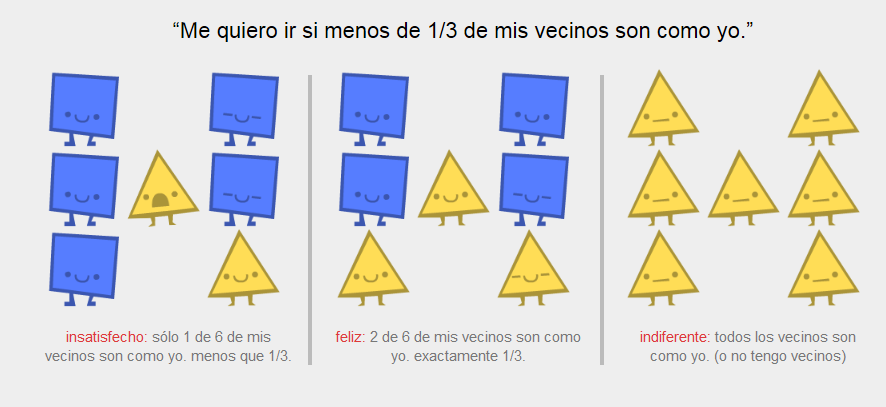
\includegraphics[width=0.9\linewidth]{figuras/Schelling_cod_4.png}
		%	\caption{}
		\label{fig:schellingcod4}
	\end{figure}
\end{frame}

\begin{frame}
	\frametitle{Modelo de Segregación de Schelling}
Ingresar a :

 \textbf{Biblioteca de Modelos / Sample Models / Social Science / Segregation}
\begin{figure}
	\centering
	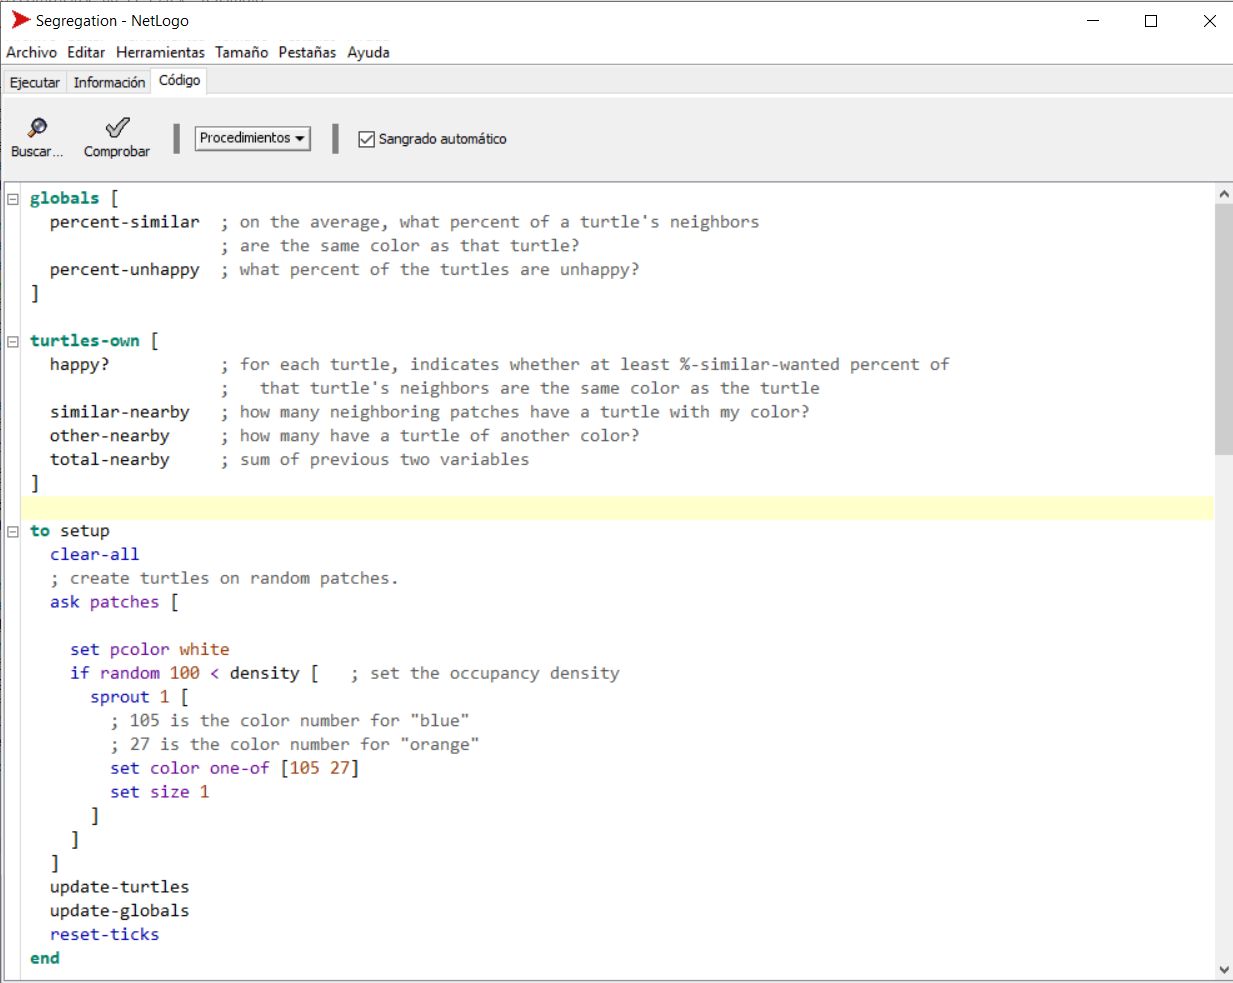
\includegraphics[width=0.75\linewidth]{figuras/Schelling_cod_1}
%	\caption{}
	\label{fig:schellingcod1}
\end{figure}
\end{frame}

\begin{frame}
	\frametitle{Modelo de Segregación de Schelling}
	\begin{figure}
		\centering
		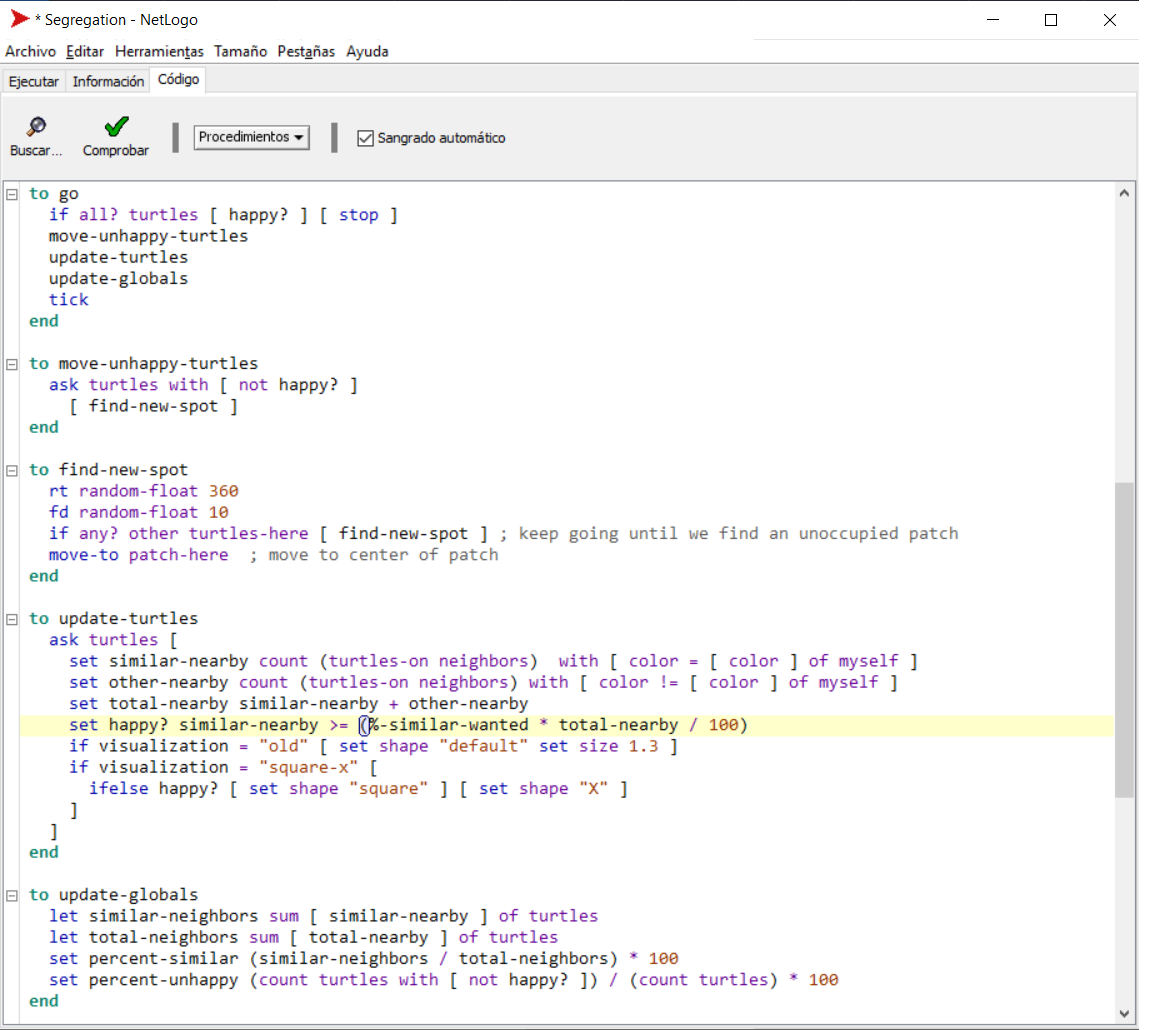
\includegraphics[width=0.7\linewidth]{figuras/Schelling_cod_2}
		%	\caption{}
		\label{fig:schellingcod2}
	\end{figure}
\end{frame}

\begin{frame}
	\frametitle{Modelo de Segregación de Schelling}
\framesubtitle{Variables globales y agentes. Clases y sub-clases.}
\begin{itemize}
	\item Debemos enunciar las variables que utilizaremos en el resto del código.
	\item No todas las variables afectan a los distintos agentes por igual. Algunas son intrínsecas a cada agente y otras afectan a todos los agentes.
	\item En este código, las variables globales son promedios en el total de la población o parámetros que se aplican a toda la población.
	\begin{itemize}
		\item \underline{density}: Proporción del total de lugares ocupados.
		\item \underline{\%-similar-wanted}: Umbral mínimo de vecinos del mismo tipo admisible.
		\item \underline{percent-similar}: Globalmente, ¿cuál es el porcentaje de los vecinos de cada agente que son del mismo color que cada agente? 
		\item \underline{percent-unhappy}: ¿qué porcentaje de la población no está conforme con el lugar donde se encuentra?
	\end{itemize}
\end{itemize}
\end{frame}

\begin{frame}
	\frametitle{Modelo de Segregación de Schelling}
	\framesubtitle{Variables globales y agentes. Clases y sub-clases. (cont.)}
	\begin{itemize}
		\item Las variables referidas a cada agente ``turtles-own'' son las siguientes:
		\begin{itemize}
			\item \underline{happy?}: si el agente está conforme con su lugar en la grilla. 
			\item \underline{similar-nearby}: ¿cuántos en mi entorno son de mi mismo \textit{tipo}?
			\item \underline{other-nearby}: ¿cuántos en mi entorno son \textit{diferentes}?
			\item \underline{total-nearby}: similar-nearby + other-nearby. Total de vecinos.
		\end{itemize}
	\item Esta es la información que tiene disponible cada agente en este modelo. En este caso, los agentes no interactúan con las variables globales.
	\end{itemize}
\end{frame}

\begin{frame}
\frametitle{Modelo de Segregación de Schelling}
\framesubtitle{Procedimientos}
\begin{itemize}
	\item SETUP
	\item GO
	\begin{itemize}
	\item move-unhappy-turtles: para indicar que si no están conformes, que utilicen el procedimiento \textit{find-new-spot}.
	\item find-new-spot: para buscar un lugar aleatoriamente.
	\item update-turtles: calcula si está conforme, a partir de observar su entorno.
	\item update-globals: se calculan las variables globales.
	\end{itemize}
\end{itemize}
\end{frame}

\begin{frame}
	\frametitle{Modelo de Segregación de Schelling}
	\begin{figure}
		\centering
		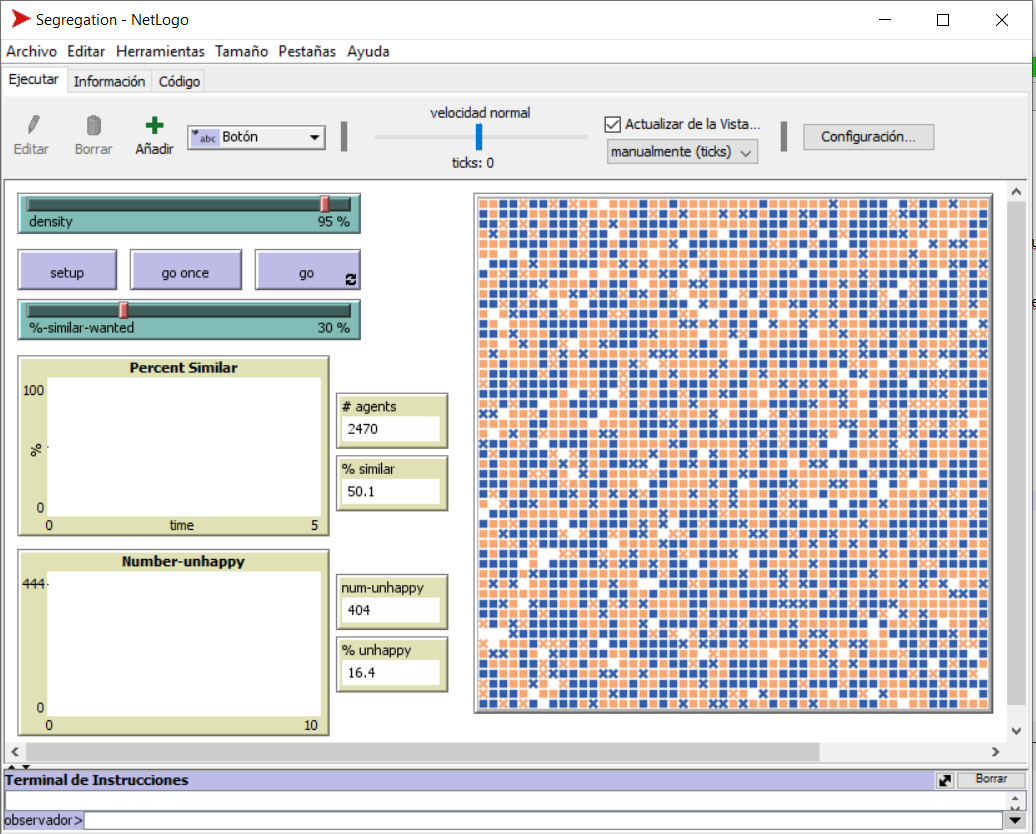
\includegraphics[width=0.9\linewidth]{figuras/Schelling_cod_3}
		%	\caption{}
		\label{fig:schellingcod3}
	\end{figure}
\end{frame}

\begin{frame}
\frametitle{Modelo de Segregación de Schelling}
\framesubtitle{Interfaz}
\begin{itemize}
	\item Las variables globales ``density'' y ``\%-similar-wanted'' pueden modificarse desde la interfaz.
	\item Los colores simbolizan los \textit{tipos}. Los agentes con forma de "X" son aquellos que no están conformes con el lugar donde se encuentran (en el próximo período, van a modificar su lugar).
	\item Se muestran gráficos de \textit{percent-similar} y \textit{percent-unhappy}.
\end{itemize}	
\end{frame}


\begin{frame}
\frametitle{Modelo de Segregación de Schelling}
Resultados:
\begin{itemize}
	\item ¿qué sucede con un límite alto? (suponemos una densidad del 90\% y un valor límite del 65\%). ¿qué sucede si llegado el final de la simulación, el umbral pasa al 30\%?.
	\item ¿y con límite más bajo? (una densidad del 97\% y un valor límite del 30\%).
	\item ¿qué podemos decir acerca de la linealidad de los parámetros?
\end{itemize}
En el último caso, no hay ningún individuo que busque un vecindario segregado; sin embargo, el resultado global es diferente.
\\ Schelling describe este proceso como los "micromotivos" que producen un "macro-comportamiento".
\end{frame}

\begin{frame}
\frametitle{Modelo de Segregación de Schelling (cont.)}
Ejemplo 1:
\begin{figure}
	\centering
	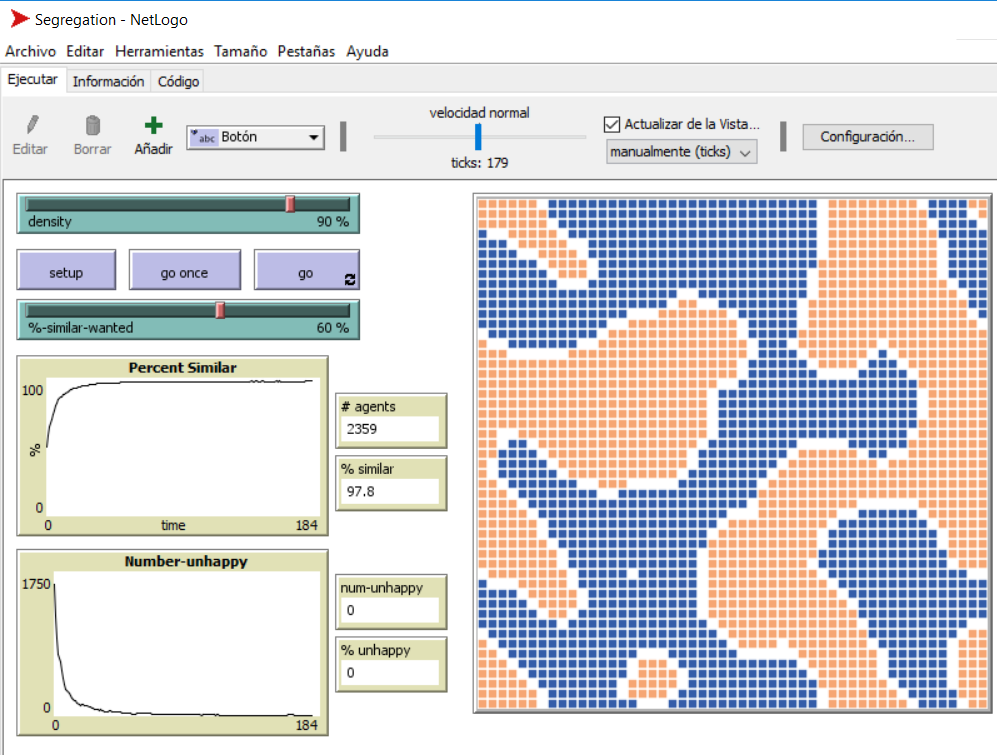
\includegraphics[width=0.7\linewidth]{figuras/Schelling_1}
	%	\caption{}
	\label{fig:schelling1}
\end{figure}
\end{frame}

\begin{frame}
\frametitle{Modelo de Segregación de Schelling (cont.)}
Ejemplo 2:
\begin{figure}
	\centering
	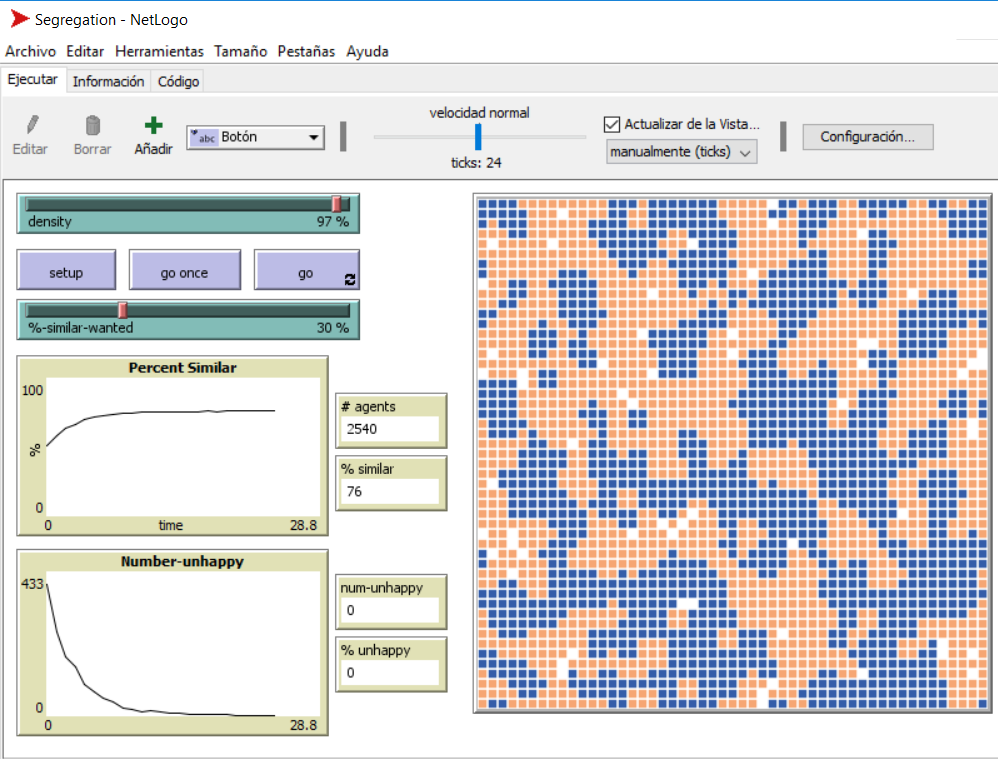
\includegraphics[width=0.7\linewidth]{figuras/Schelling_2}
	%	\caption{}
	\label{fig:schelling2}
\end{figure}
\end{frame}

\begin{frame}
	\frametitle{modelo de Schelling}
	\framesubtitle{algunos experimentos}
\begin{enumerate}
\small	\item La proporción de individuos insatisfechos disminuye en el tiempo. ¿qué podemos decir acerca de la velocidad? (calcular con un umbral mínimo del 40\% y una densidad del 98\%) \textbf{(ver ``experiment1'' en BehaviorSpace)}.
	\item ¿Para qué valores de los parámetros este modelo no converge (establecer un máximo t=1000)? \textbf{(ver ``experiment2'' en BehaviorSpace)}.	
	\item ¿Los resultados cambian (conformación de grupos bien definidos, segregación) si establecemos un límite máximo a la cantidad de vecinos similares? Establecer valores máximos entre 60\% y 90\% y mínimos entre 0\% y 30\%, con una densidad del 85\%. \textbf{(ver ``experiment3'' en BehaviorSpace).}
\end{enumerate}	
\vspace{0.6cm}
$\longrightarrow$ \large ¿resultados?
\end{frame}

\begin{frame}
	\frametitle{Modelo de Schelling}
Algunas ideas:
\begin{itemize}
	\item Pequeñas tendencias individuales llevan a grandes tendencias colectivas. El problema de la segregación en esta sociedad simulada no es por culpa de todos o de algunos ``extremistas''. El ``culpable'' es el proceso de interacción.
	\item Alta dependencia temporal. La segregación no disminuye sólo con una caída del umbral, sino que son necesarias otras acciones.
	\item Demanda por diversidad. Para favorecer a la diversidad, tal vez sea una buena alternativa establecer valores máximos para los \textit{similares} en el entorno.
\end{itemize}

\end{frame}

\begin{frame}
\frametitle{Ejemplo: Modelo de Schelling (cont.)}
\framesubtitle{Estudios empíricos surgidos a partir del modelo de Schelling} 
\begin{figure}
	\centering
	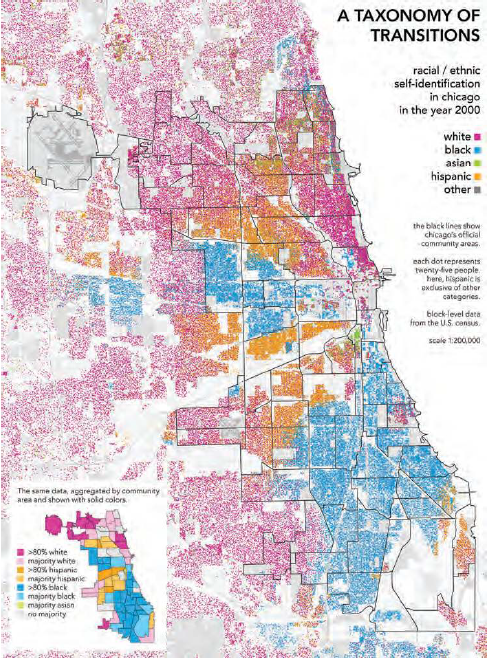
\includegraphics[width=0.5\linewidth]{figuras/Schelling_3}
	%	\caption{}
	\label{fig:schelling3}
\end{figure}
\end{frame}

\begin{frame}
\small
	\frametitle{Ejemplo: Modelo de Schelling (cont.)}
	\framesubtitle{Estudios empíricos surgidos a partir del modelo de Schelling} 
\begin{itemize}
    \item Mapa de la segregación en ciudades de Estados Unidos (en base al censo de 2015):
\url{https://www.nytimes.com/interactive/2015/07/08/us/census-race-map.html}
\item Mapa de la segregación en ciudades de Estados Unidos (en base al censo de 2020):
\url{https://edition.cnn.com/interactive/2021/us/census-race-ethnicity-map/}
\item Para Europa: \url{https://www.bloomberg.com/news/articles/2015-11-16/europe-s-cities-are-suffering-from-economic-segregation-and-inequality-too}\\
\item \url{https://www.residentialsegregation.org/research-findings}
\end{itemize}


\end{frame}


\begin{frame}
	\frametitle{Ejemplo: un mercado inmobiliario\footnote{Heymann et al. (2013; pp 85-87). Economía de fronteras abiertas: exploraciones en sistemas sociales complejos. Teseo.}}
\begin{itemize} \small
	\item Las mudanzas implican una transacción económica
	\item Los agentes toman en cuenta el costo de trasladarse a un barrio más afín.
	\item Se define la utilidad del agente $i$ con capital $K_i$ y una propiedad de valor $P_i$ como $U_i\sim K_i^{\alpha}P_i^{1-\alpha}$.
	\item El valor que le asigna a una propiedad se encuentra definida por su entorno:
	\begin{itemize} \footnotesize
		\item $P(X)=A[C(X)-C(\hat{X})]+B$ (alternativa 1)
		\item $P(X)=A[C(\hat{X})- C(X)]+B$ (alternativa 2), donde C(X) es la cantidad de agentes del color "X" en su vecindad. A y B ctes. 
	\end{itemize}
\item La dinámica implica que:
\begin{itemize} \footnotesize
	\item  se eligen dos agentes al azar y cada uno calcula lo que pagaría por la propiedad del otro, 
	\item se determina un precio de transacción por el promedio
	\item intercambian si pueden pagar la diferencia y si ambos mejoran su utilidad.
\end{itemize}	
\end{itemize}
\end{frame}

\begin{frame}
	\frametitle{Ejemplo: un mercado inmobiliario (cont.)}
	\begin{figure}
		\centering
		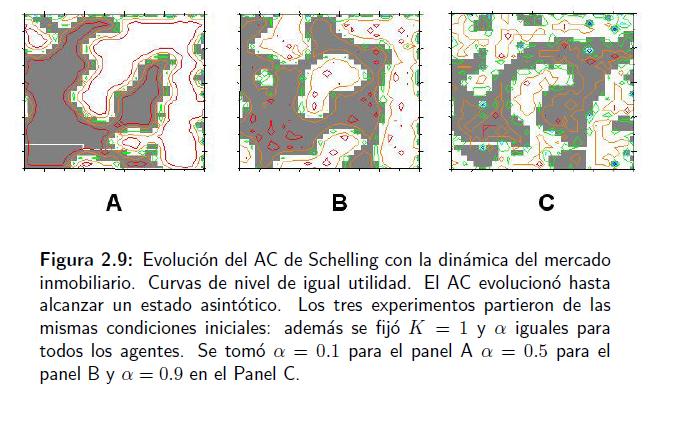
\includegraphics[width=0.9\linewidth]{figuras/Schelling_cod_5}
		%	\caption{}
		\label{fig:schelling5}
	\end{figure}
\end{frame}

\end{document}

